% PHYS1600J Project Template based on RevTeX 4.2.
% The document class and two-column visual structure are retained from the
% supplied course template; only standard packages needed by this paper are added.
\documentclass[reprint,floatfix]{revtex4-2}

\usepackage{graphicx}
\usepackage{geometry}
\usepackage{subfigure}
\usepackage{amsfonts,amsmath,amssymb}
\usepackage{enumerate}
\usepackage{dcolumn}
\usepackage{bm}
\usepackage{booktabs}
\usepackage{multirow}
\usepackage{siunitx}
\usepackage{xcolor}
\usepackage{microtype}
\usepackage{placeins}
\usepackage{xurl}
\usepackage[colorlinks,citecolor=black,urlcolor=black,linkcolor=black]{hyperref}
\usepackage[mathlines]{lineno}

\sisetup{separate-uncertainty=true,per-mode=symbol,range-phrase=--,range-units=single}
\graphicspath{{../figures/}}
\newcommand{\dd}{\mathrm{d}}
\newcommand{\e}{\mathrm{e}}
\newcommand{\vect}[1]{\bm{#1}}


\begin{document}

\title{Problem B\\The Measure-Zero Home Run: From an Ideal Surface Orbit to a Real Lunar Ballpark}

% Replace the three placeholders below before submission.
\author{Student I}
\email{student1@sjtu.edu.cn}
\author{Student II}
\email{student2@sjtu.edu.cn}
\author{Student III}
\email{student3@sjtu.edu.cn}
\affiliation{UM-SJTU Joint Institute, Shanghai Jiao Tong University, Shanghai 200240, China}

\begin{abstract}
Could a baseball struck on the Moon orbit once and hit the batter from behind? We answer this question through a hierarchy of analytic and numerical models. For a smooth, nonrotating spherical Moon, the circular and escape speeds at the mean radius are \SI{1.680}{km.s^{-1}} and \SI{2.376}{km.s^{-1}}. We prove that a ball launched exactly from the reference surface can remain outside the Moon for a complete bound revolution only if it is launched tangentially with $1\leq u=v/v_c<\sqrt{2}$. Thus the admissible set has zero area in speed--angle space even though a one-parameter family of mathematical solutions exists. A finite ball-centre height opens a narrow safe wedge: at a \SI{1}{m} launch height and $u=1.2$, the maximum elevation magnitude is only \SI{0.0340}{deg}. The fastest recorded Major League Baseball exit speed is approximately \SI{54.9}{m.s^{-1}}, a factor of 30.6 below lunar circular speed, so no unaided human hit is remotely orbital. Lunar rotation changes the conclusion about ``return'': during a near-surface \SI{108.31}{min} orbit, an equatorial field moves about \SI{30.05}{km}, whereas a polar field has no translational rotation miss. Exact multi-orbit resonances exist in the ideal model but occur near terrain-threatening low altitudes. Finally, a degree-2 lunar gravity model produces a \SI{9.5}{km} one-period displacement from the central-gravity prediction for a representative \SI{20}{km}-altitude case; Earth and solar tides provide smaller short-arc corrections. We combine these results with LOLA topography and GRAIL gravity data products to propose terrain-safe numerical tests and a three-dimensional lunar baseball rule set. The orbital home run is mathematically possible, physically launcher-dependent, dynamically fragile, and unsuitable for ordinary open-field baseball.
\begin{description}
    \item[Keywords] lunar orbit, two-body dynamics, sensitivity analysis, lunar gravity, baseball physics.
\end{description}
\end{abstract}

\maketitle

\section{Introduction}

\subsection{Background and motivation}

On Earth, a home run is a short atmospheric flight whose outcome is governed by the ball--bat collision, aerodynamic drag, lift, spin, and the geometry of a local field \cite{Nathan2000,Adair2002}. The lunar version reverses the hierarchy of effects. With no appreciable atmosphere, aerodynamic forces disappear to leading order, while the curvature of the Moon and the inverse-square variation of gravity become essential. A sufficiently fast baseball is therefore not a projectile in a uniform gravitational field; it is a satellite.

The question appears at first to require only the lunar ``first cosmic velocity.'' That calculation is necessary but not sufficient. A meaningful self-hitting home run must satisfy four distinct conditions:
\begin{enumerate}
    \item the trajectory must be bound to the Moon;
    \item it must not intersect the lunar surface or terrain before completing a revolution;
    \item it must return to the moving ballpark, not merely to the original point in an inertial frame;
    \item the result must remain valid under realistic uncertainties and gravitational perturbations.
\end{enumerate}
These distinctions motivate a model hierarchy rather than a single calculation.

\subsection{Problem restatement}

We model a baseball launched from radius $r_0=R+h$ with surface-relative speed $v_s$, flight-path angle $\gamma$ measured above the local horizontal, azimuth $A$ measured clockwise from north, and launch latitude $\phi$. We seek combinations of speed, angle, and altitude that permit at least one complete lunar revolution and a return to the batter. We then quantify sensitivity to the initial state; add altitude, lunar rotation, terrain, non-spherical lunar gravity, and third-body tides; and use the results to discuss a fair and safe lunar baseball rule set.

The phrase ``return to the batter'' is used carefully. In a static central field, every collision-free bound Kepler orbit returns exactly to its initial phase-space state after one period. In a rotating and irregular lunar environment, the relevant quantity is instead the distance between the ball and the rotating launch site at the candidate return time.

\subsection{Main contributions}

The work makes six connected contributions.
\begin{enumerate}
    \item We prove a \emph{surface-launch theorem}: in the ideal spherical model, a collision-free bound orbit launched exactly at the surface requires $\gamma=0$ and $1\leq v/v_c<\sqrt{2}$.
    \item We derive closed-form orbital altitude and period formulae, and an exact relation between angular launch error and the early re-impact point.
    \item We generalize the existence condition to arbitrary launch height and arbitrary terrain-envelope radius, revealing how finite height opens a narrow but nonzero feasible region.
    \item We separate inertial closure from rotating-site closure, identify the polar exception, and construct exact ideal multi-orbit resonances.
    \item We compare central, degree-2 lunar gravity, terrestrial-tide, and solar-tide propagations against a verified analytic benchmark.
    \item We formulate a terrain-safe orbital-corridor test and a three-dimensional definition of a fair lunar ball.
\end{enumerate}

\section{Notation, data, and dimensionless parameters}

\subsection{Notation}

\begin{table}[hbt]
\caption{Principal notation. Angles are in radians unless stated otherwise.}
\label{tab:notation}
\resizebox{\columnwidth}{!}{%
\begin{ruledtabular}
\begin{tabular}{ll}
Symbol & Meaning \\
\hline
$\mu$ & lunar gravitational parameter \\
$R$ & mean lunar reference radius \\
$r_0=R+h$ & ball-centre launch radius \\
$R_t$ & required obstacle-envelope radius \\
$v,\ v_s$ & inertial and surface-relative launch speeds \\
$v_c,\ v_{\rm esc}$ & circular and escape speeds at $R$ \\
$u=v/v_c$ & dimensionless inertial launch speed \\
$\gamma$ & flight-path angle above local horizontal \\
$A$ & launch azimuth, clockwise from north \\
$a,e,p$ & semimajor axis, eccentricity, semilatus rectum \\
$r_p,r_a$ & periapsis and apoapsis radii \\
$T$ & osculating orbital period \\
$\Omega$ & lunar sidereal rotation rate \\
$\phi,\lambda$ & body-fixed latitude and longitude \\
$J_2,C_{22}$ & unnormalised degree-2 gravity coefficients
\end{tabular}
\end{ruledtabular}%
}
\end{table}

\subsection{Physical constants and data provenance}

For reproducibility, all calculations use SI units internally. The central value $\mu=\SI{4.902800118e12}{m^3.s^{-2}}$ and mean radius $R=\SI{1737.4}{km}$ are consistent with JPL lunar parameters and modern ephemerides \cite{Park2021,JPLParameters}. The derived surface acceleration, \SI{1.6242}{m.s^{-2}}, is close to the rounded \SI{1.62}{m.s^{-2}} supplied in the problem. The lunar sidereal rotation period is \SI{27.321661}{day} \cite{Archinal2018,NASAMoonRotation}.

Topography is referenced to the LOLA global digital elevation products \cite{Smith2010,PDSLOLA}. The packaged workflow records two useful scales: the \SI{0.25}{deg} LDEM4 grid spans approximately $-\SI{8.879}{km}$ to $+\SI{10.504}{km}$ relative to the \SI{1737.4}{km} sphere, while finer LOLA/LROC analyses place the global high point near \SI{10.8}{km} \cite{LROCHighPoint}. Non-spherical lunar gravity is motivated by the GRAIL GRGM900C and later degree-1200 products \cite{Lemoine2014,Goossens2020,PDSGRAIL}. The default package uses only degree-2 coefficients so that it remains small and independently reproducible; scripts and official links for the larger products are supplied.

A representative baseball mass $m_b=\SI{0.145}{kg}$ and radius $r_b=\SI{0.0369}{m}$ are used. For a human-scale benchmark, the fastest recorded Statcast home-run exit speed is approximately \SI{122.9}{mph}, or \SI{54.94}{m.s^{-1}} \cite{MLBCruz2026}.

\begin{table*}[hbt]
\caption{Reference constants and derived ideal quantities. The number of significant figures shown is greater than needed for physical prediction but is useful for code verification.}
\label{tab:constants}
\begin{ruledtabular}
\begin{tabular}{lccc}
Quantity & Symbol & Value & Source or definition \\
\hline
Lunar gravitational parameter & $\mu$ & \SI{4.902800118e12}{m^3.s^{-2}} & JPL/DE440 \\
Mean lunar radius & $R$ & \SI{1.737400e6}{m} & LOLA/JPL reference \\
Surface gravity & $\mu/R^2$ & \SI{1.624219}{m.s^{-2}} & derived \\
Surface circular speed & $v_c$ & \SI{1679.857}{m.s^{-1}} & $\sqrt{\mu/R}$ \\
Surface escape speed & $v_{\rm esc}$ & \SI{2375.676}{m.s^{-1}} & $\sqrt{2\mu/R}$ \\
Surface circular period & $T_c$ & \SI{6498.416}{s} & $2\pi\sqrt{R^3/\mu}$ \\
Sidereal rotation period & $P_M$ & \SI{2360591.5}{s} & IAU/NASA \\
Equatorial rotation speed & $\Omega R$ & \SI{4.6244}{m.s^{-1}} & derived \\
Global terrain scale & $H_{\max}$ & \SI{10.786}{km} & LOLA/LROC scale
\end{tabular}
\end{ruledtabular}
\end{table*}

\subsection{Dimensionless control parameters}

The problem is organized by a small set of dimensionless quantities:
\begin{align}
 u&=\frac{v}{v_c}, \qquad \eta=\frac{h}{R},\\
 \tau&=\frac{H_{\max}}{R}, \qquad \rho=\frac{\Omega R}{v_c}.
\label{eq:dimensionless}
\end{align}
For the Moon, $\tau\simeq6.21\times10^{-3}$ and $\rho\simeq2.75\times10^{-3}$. The first controls the energetic orbit family, $\eta$ controls the angular opening of the feasible set, $\tau$ measures terrain importance, and $\rho$ measures the difference between inertial and surface-relative launch speeds. Perturbation strengths are represented by $J_2\simeq2.03\times10^{-4}$, $C_{22}\simeq2.24\times10^{-5}$, and the local ratios of third-body tidal acceleration to central lunar gravity.

\section{Assumptions and model hierarchy}

The assumptions are introduced in stages so that every additional physical effect has a measurable purpose.

\begin{table*}[hbt]
\caption{Model hierarchy. ``Return'' in M0 means inertial phase-space closure; in M1--M4 it means proximity to the rotating launch site.}
\label{tab:models}
\small
\resizebox{\textwidth}{!}{%
\begin{ruledtabular}
\begin{tabular}{clll}
Model & Added physics & Main question & Validation \\
\hline
M0 & spherical static Moon; central gravity & collision-free closed orbit? & analytic Kepler solution \\
M1 & finite height, site geometry, rotation & return to moving field? & frames and resonances \\
M2 & LOLA terrain envelope or DEM & clear actual topography? & clearance event test \\
M3 & rotating degree-2 lunar gravity & is Kepler closure stable? & step and conservation checks \\
M4 & Earth and Sun differential tides & are third bodies relevant? & trajectory differences
\end{tabular}
\end{ruledtabular}%
}
\end{table*}

The ideal model treats the ball as a point mass after impact, neglects air resistance, and neglects the ball's spin. These approximations are unusually strong on Earth but appropriate on the Moon: without an atmosphere, spin produces no Magnus force. The lunar exosphere is so tenuous that drag is negligible on a roughly two-hour arc \cite{NASALunarAtmosphere}. We also neglect solar radiation pressure in the default propagation. Even with a conservative area-to-mass ratio $A/m\sim\SI{0.03}{m^2.kg^{-1}}$, its acceleration is only of order $10^{-7}$--$10^{-6}\,\si{m.s^{-2}}$, below the degree-2 lunar correction and comparable to the small solar tidal term. It can be added in a later high-fidelity study.

The Moon is first treated as a rigid uniformly rotating body. Physical libration and detailed attitude are omitted from M1--M4; SPICE kernels would be the natural extension \cite{Acton1996}. For the one-orbit third-body comparison, Earth and Sun directions are held fixed. Their directions change only modestly during a two-hour low lunar orbit, so the approximation is sufficient for an order-of-magnitude error budget but not for multi-day resonant trajectories.

\section{Pure ideal case: the spherical nonrotating Moon}

\subsection{Governing equations}

In a Moon-centred inertial frame the point-mass equation is
\begin{equation}
 \ddot{\vect r}=-\frac{\mu}{r^3}\vect r.
\label{eq:twobody}
\end{equation}
The conserved specific energy and angular momentum are
\begin{equation}
 \mathcal E=\frac{v^2}{2}-\frac{\mu}{r},\qquad
 \vect H=\vect r\times\vect v.
\label{eq:invariants}
\end{equation}
Bound motion requires $\mathcal E<0$. Standard two-body relations give \cite{Bate1971,Curtis2020,Vallado2013}
\begin{equation}
 a=-\frac{\mu}{2\mathcal E},\qquad
 p=\frac{H^2}{\mu},\qquad
 r(f)=\frac{p}{1+e\cos f}.
\label{eq:conic}
\end{equation}

\subsection{Surface-launch theorem}

\textbf{Theorem.} Consider a ball launched from exactly $r=R$ in the ideal model. It completes a bound revolution without entering $r<R$ if and only if
\begin{equation}
 \boxed{\gamma=0,\qquad 1\leq u<\sqrt{2}.}
\label{eq:surface_theorem}
\end{equation}

\emph{Proof.} A collision-free trajectory beginning at the minimum allowed radius must have the launch point as a radial turning point, so $\dot r(0)=v\sin\gamma=0$. Hence $\gamma=0$ (the inward solution is immediately excluded). A horizontal launch at $R$ is a periapsis only when the tangential speed is at least the circular speed, $v\geq v_c$. Finally, the orbit is bound only for $v<v_{\rm esc}=\sqrt{2}v_c$. Conversely, every horizontal launch satisfying these inequalities has $r_p=R$ and a bound conic, so $r\geq R$ for the full period. \hfill$\square$

This result is more informative than the circular-speed calculation. In the two-dimensional $(u,\gamma)$ plane, the feasible set is a line segment and therefore has zero area. There are infinitely many ideal solutions, but no open neighbourhood of robust surface-launch solutions. The $u=1$ circular case lies exactly on the reference sphere and has zero clearance; a finite-size ball, terrain, or any modelling error makes this boundary physically unacceptable.

\subsection{Closed-form orbit family}

For a horizontal launch from $R$ with $1\leq u<\sqrt{2}$,
\begin{align}
 a&=\frac{R}{2-u^2}, \qquad e=u^2-1,\label{eq:ae}\\
 r_p&=R, \qquad r_a=R\frac{u^2}{2-u^2},\label{eq:rpra}\\
 T&=T_c(2-u^2)^{-3/2}.\label{eq:period_u}
\end{align}
The required speed rises only from $v_c$ to $\sqrt{2}v_c$, but the apoapsis and period diverge as escape is approached. Figure~\ref{fig:family} shows this singular behaviour, and Table~\ref{tab:ideal_cases} gives benchmark cases used to verify the scripts.

\begin{figure*}[hbt]
\centering
\subfigure[Apoapsis altitude.]{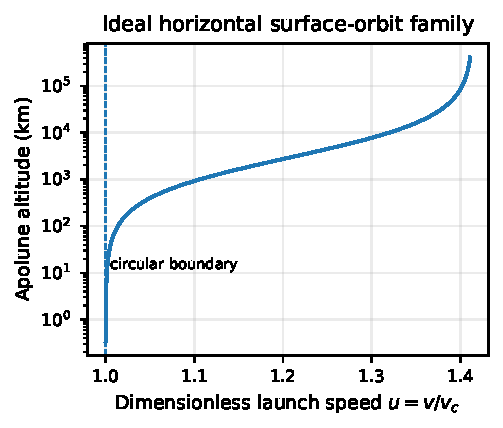
\includegraphics[width=0.47\textwidth]{fig01_orbit_family_altitude.pdf}}
\hfill
\subfigure[Orbital period.]{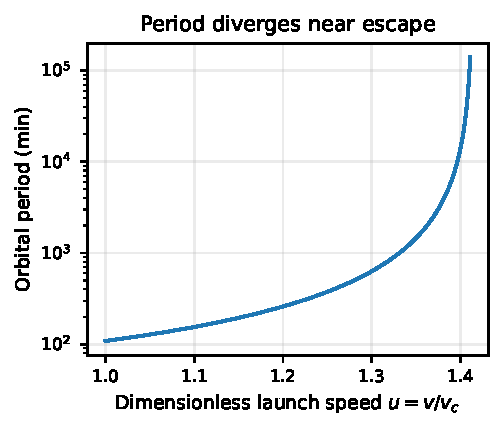
\includegraphics[width=0.47\textwidth]{fig02_orbit_family_period.pdf}}
\caption{The ideal horizontal surface-orbit family. Close to $u=1$ the orbit is low and fast; close to $\sqrt 2$, its scale becomes incompatible with a Moon-only two-body approximation.}
\label{fig:family}
\end{figure*}

\begin{table}[hbt]
\caption{Ideal horizontal reference cases.}
\label{tab:ideal_cases}
\begin{ruledtabular}
\begin{tabular}{cccc}
$u$ & $v$ (\si{km.s^{-1}}) & $h_a$ (km) & $T$ (min) \\
\hline
1.001 & 1.6815 & 6.97 & 108.63 \\
1.010 & 1.6967 & 71.3 & 111.66 \\
1.050 & 1.7638 & 396.8 & 127.38 \\
1.100 & 1.8478 & 923.7 & 154.25 \\
1.200 & 2.0158 & 2730 & 258.45 \\
1.300 & 2.1838 & 7734 & 627.50
\end{tabular}
\end{ruledtabular}
\end{table}

The label ``low lunar orbit'' should therefore not be applied to the whole interval. Near escape, the apoapsis reaches many lunar radii and Earth perturbations can no longer be treated as small. Later realistic comparisons deliberately use a much lower orbit.

\subsection{Energetic plausibility of a human hit}

The fastest recorded MLB home-run exit speed, \SI{54.94}{m.s^{-1}}, is only
\begin{equation}
 \frac{v_{\rm MLB}}{v_c}=0.0327,
\end{equation}
so lunar circular speed is larger by a factor of 30.6. Because kinetic energy scales as $v^2$, a \SI{0.145}{kg} ball at $v_c$ carries about \SI{205}{kJ}, compared with \SI{219}{J} at the Statcast benchmark: a factor of approximately 935. A human batter cannot supply the required speed. The rest of the paper therefore treats the ``hitter'' as an ideal launcher or future impact system and asks whether the orbital geometry itself is possible.

\section{Sensitivity and reasonableness of the ideal solution}

\subsection{Exact early-impact relation for a surface launch}

The zero-measure result can be made quantitative. At $r=R$, let the launch flight-path angle be a small positive $\gamma$. The eccentricity-vector relations give
\begin{align}
 e\cos f_0&=u^2\cos^2\gamma-1,\label{eq:ecos}\\
 e\sin f_0&=u^2\sin\gamma\cos\gamma,\label{eq:esin}
\end{align}
where $f_0$ is the launch true anomaly measured from periapsis. Hence
\begin{equation}
 \tan f_0=\frac{u^2\sin\gamma\cos\gamma}
 {u^2\cos^2\gamma-1}.
\label{eq:f0}
\end{equation}
The second intersection with the same sphere occurs at $-f_0$ modulo $2\pi$, so the trajectory falls short of a full revolution by $2f_0$. The corresponding surface-arc shortfall is
\begin{equation}
 s=2Rf_0\simeq2R\frac{u^2}{u^2-1}|\gamma|,
 \qquad |\gamma|\ll1.
\label{eq:shortfall}
\end{equation}

\begin{figure}[hbt]
\centering
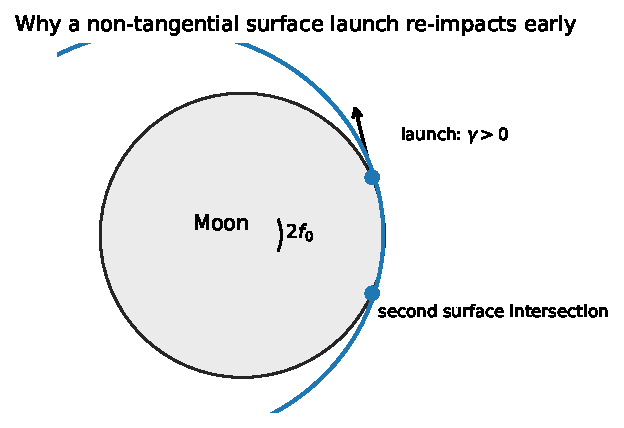
\includegraphics[width=0.47\textwidth]{fig03_surface_intersection_geometry.pdf}
\caption{A non-tangential launch from the reference sphere intersects the sphere again before completing $2\pi$. The angular shortfall is $2f_0$.}
\label{fig:geometry}
\end{figure}

Figure~\ref{fig:angle_sensitivity} compares Eq.~\eqref{eq:shortfall} with the exact relation. At $u=1.2$, the proportionality factor is about \SI{1.14e7}{m.rad^{-1}}. In the strict $h=0$ model, any nonzero angular error causes premature impact; the plotted distance indicates where it happens, not a finite safe tolerance.

\begin{figure}[hbt]
\centering
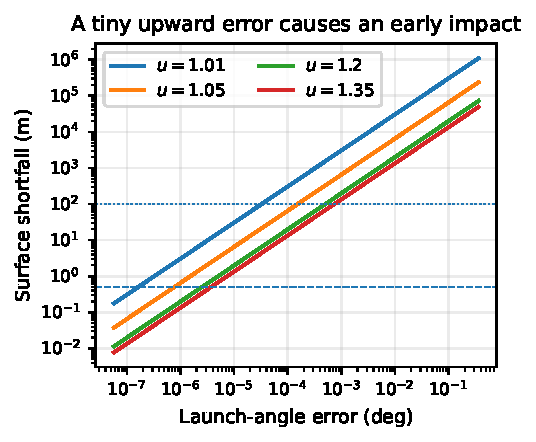
\includegraphics[width=0.47\textwidth]{fig04_angle_sensitivity.pdf}
\caption{Exact surface shortfall as a function of upward launch-angle error. Near $u=1$, a fixed angular error is especially damaging because the ellipse has very small radial clearance.}
\label{fig:angle_sensitivity}
\end{figure}

\subsection{Finite launch height: a nonzero but narrow safe wedge}

A real ball centre is above the ground, a batter may strike from a platform, and a mountaintop has $r_0>R$. Let $R_t$ denote the radius of the obstacle envelope to be cleared. For a launch at $r_0$ with speed $v$ and angle $\gamma$, the specific angular momentum is
\begin{equation}
 H=r_0v\cos\gamma.
\end{equation}
At the boundary of safety, the osculating periapsis is exactly $R_t$. Equating the energy at launch and periapsis gives
\begin{equation}
 v^2\left(r_0^2\cos^2\gamma-R_t^2\right)
 =2\mu R_t\left(1-\frac{R_t}{r_0}\right).
\label{eq:height_boundary}
\end{equation}
Thus a bound collision-free orbit requires
\begin{equation}
 v^2\left(r_0^2\cos^2\gamma-R_t^2\right)
 \geq2\mu R_t\left(1-\frac{R_t}{r_0}\right),
\label{eq:height_inequality}
\end{equation}
plus $v<\sqrt{2\mu/r_0}$. The minimum speed for a selected angle is
\begin{equation}
 v_{\min}=\left[
 \frac{2\mu R_t(1-R_t/r_0)}
 {r_0^2\cos^2\gamma-R_t^2}
 \right]^{1/2}.
\label{eq:vmin}
\end{equation}
For $R_t=R$, $r_0=R+h$, and $v=u_0\sqrt{\mu/r_0}$, a small-height expansion gives
\begin{equation}
 |\gamma|_{\max}\simeq
 \left[\frac{2h}{R}\left(1-\frac{1}{u_0^2}\right)\right]^{1/2}.
\label{eq:gamma_height}
\end{equation}
The square-root dependence is important: increasing the launch height by a factor of 100 improves angular tolerance by only a factor of 10.

At $h=\SI{1}{m}$ and $u_0=1.2$, the exact tolerance is \SI{0.03398}{deg}. If only the ball radius $h=r_b=\SI{0.0369}{m}$ is credited, it drops to about \SI{0.0065}{deg}. Figure~\ref{fig:height_tolerance} maps the tolerance over seven orders of magnitude in height.

\begin{figure}[hbt]
\centering
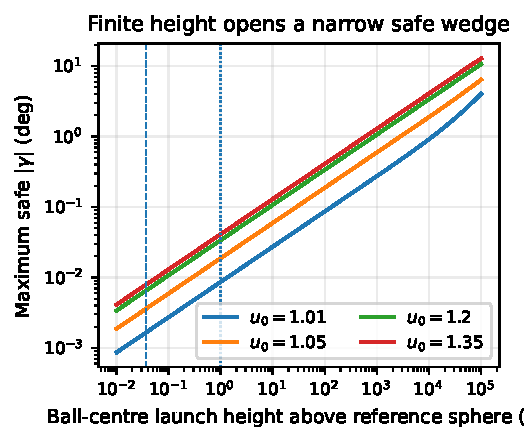
\includegraphics[width=0.47\textwidth]{fig05_finite_height_tolerance.pdf}
\caption{Maximum angle magnitude that keeps the osculating periapsis above the mean sphere. The dashed marker is one ball radius; the dotted marker is a \SI{1}{m} launch height.}
\label{fig:height_tolerance}
\end{figure}

\subsection{Speed sensitivity}

For $u=1+\delta$ with $\delta\ll1$, Eq.~\eqref{eq:rpra} gives
\begin{equation}
 h_a=r_a-R\simeq4R\delta
 =4R\frac{\Delta v}{v_c}.
\label{eq:ha_sensitivity}
\end{equation}
Near circular speed, an additional \SI{1}{m.s^{-1}} therefore raises the ideal apoapsis by approximately \SI{4.14}{km}. The period sensitivity follows from Eq.~\eqref{eq:period_u}:
\begin{equation}
 \frac{\dd\ln T}{\dd u}=\frac{3u}{2-u^2}.
\label{eq:period_sensitivity}
\end{equation}
At $u=1.2$, a speed-ratio error of $10^{-3}$ changes the period by roughly $0.77\%$, which becomes a significant longitude error when the Moon rotates beneath the orbit.

The sensitivities separate naturally:
\begin{itemize}
    \item $\gamma$ controls whether a low-clearance trajectory intersects the surface;
    \item $v$ controls radial scale and period;
    \item in the exact central model, neither changes the one-period inertial return point for a surviving bound orbit;
    \item after rotation or perturbations are added, period and orbital-plane errors become return-position errors.
\end{itemize}
This last point prevents a common misinterpretation of Monte Carlo results: a wide inertial return cloud in the ideal two-body model would indicate a numerical or event-definition error, not physical sensitivity.

\subsection{Monte Carlo survival test}

We sampled $10^5$ launches from a \SI{1}{m} platform with nominal $u_0=1.2$, Gaussian $\sigma_u=5\times10^{-4}$, and $\sigma_\gamma=\SI{0.05}{deg}$. A launch is labelled safe only if its osculating periapsis is at or above $R$. The survival fraction is $0.503$, consistent with an analytic angular boundary of \SI{0.03398}{deg}. Figure~\ref{fig:montecarlo} shows the sharp periapsis boundary. This calculation is not a model of a particular player's biomechanics; it demonstrates how a specified launch distribution maps into a physically meaningful failure probability.

\begin{figure}[hbt]
\centering
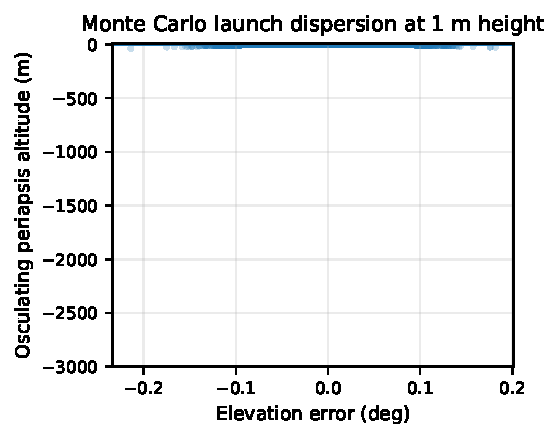
\includegraphics[width=0.47\textwidth]{fig06_monte_carlo_periapsis.pdf}
\caption{A subset of the Monte Carlo trials. Negative periapsis altitude means the osculating ellipse intersects the mean sphere.}
\label{fig:montecarlo}
\end{figure}

\section{Actual lunar conditions}

\subsection{Launch altitude, mountains, and terrain}

A mountain helps in two ways: it raises the ball centre and may provide an unobstructed local tangent. It does \emph{not} substantially reduce the required speed. For a horizontal launch only \SI{1}{m} above a conservative global envelope at $R_t=R+\SI{10.786}{km}$, Eq.~\eqref{eq:vmin} gives approximately \SI{1.675}{km.s^{-1}}, still 30 times the human exit-speed benchmark. At an altitude of \SI{20}{km}, the conservative minimum horizontal speed for clearing the same envelope is about \SI{1.668}{km.s^{-1}}.

The highest mountain is not automatically the best ballpark. Safety depends on the entire ground track, not only the launch point. Given a digital elevation model $H(\phi,\lambda)$, define the instantaneous clearance
\begin{equation}
 C(t)=r(t)-R-H[\phi(t),\lambda(t)]-r_b.
\label{eq:clearance}
\end{equation}
A terrain-safe trajectory satisfies $\min C(t)>0$. This leads to an explicit orbital-corridor optimization problem:
\begin{equation}
 \max_{\phi_0,\lambda_0,A,v,\gamma}
 \left\{\min_{0<t<T} C(t)\right\},
\label{eq:corridor}
\end{equation}
subject to a bound orbit, a return tolerance, and launcher constraints. Equation~\eqref{eq:corridor} is a more rigorous design objective than simply launching from the highest point. The packaged terrain script operates in two modes: a conservative global envelope requiring no large file, and an optional full-grid LOLA LDEM4 mode downloaded from NASA PDS.

\begin{figure}[hbt]
\centering
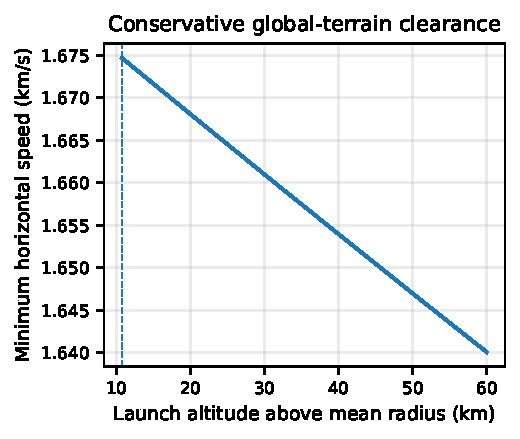
\includegraphics[width=0.47\textwidth]{fig11_terrain_envelope_speed.pdf}
\caption{Minimum horizontal speed when the complete orbit is conservatively required to remain above the global terrain-envelope radius. Mountain-scale changes in altitude barely change the orbital-speed requirement.}
\label{fig:terrain}
\end{figure}

\subsection{Lunar rotation and the moving ballpark}

In a body-fixed local frame the launch velocity is $\vect v_s$, but the inertial initial velocity is
\begin{equation}
 \vect v=\vect v_s+\vect\Omega\times\vect r_0.
\label{eq:rotation_velocity}
\end{equation}
At the equator, an eastward hit receives only \SI{4.624}{m.s^{-1}} from lunar rotation, a $0.275\%$ correction to $v_c$. The energetic benefit is small. The positional effect is not.

If a central-gravity orbit closes inertially after period $T$, the launch site has rotated through $\Delta\lambda=\Omega T$. At latitude $\phi$, the surface arc and chord distances between the old and new site positions are
\begin{align}
 s_{\rm rot}&=R|\cos\phi|\,|\Omega T|,\label{eq:rot_arc}\\
 d_{\rm rot}&=2R|\cos\phi|\left|\sin\frac{\Omega T}{2}\right|.
\label{eq:rot_chord}
\end{align}
For $T_c=\SI{108.31}{min}$, an equatorial field moves through $0.991^\circ$, corresponding to an arc of \SI{30.05}{km}. A one-orbit inertial return is therefore not a self-hit at ordinary latitudes.

\begin{figure}[hbt]
\centering
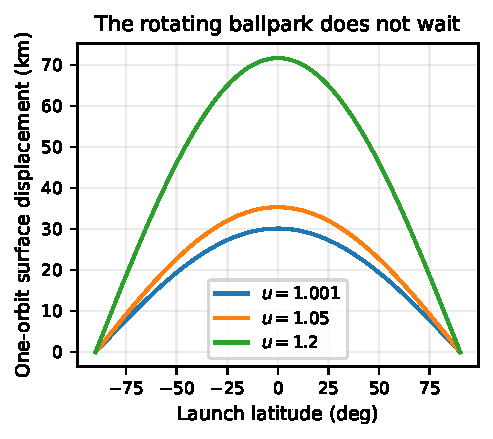
\includegraphics[width=0.47\textwidth]{fig07_rotation_miss_by_latitude.pdf}
\caption{Surface displacement of the ballpark during one ideal orbit. The translational miss vanishes at the rotation poles, making a polar ballpark a genuine special case.}
\label{fig:rotation_lat}
\end{figure}

The poles are an important exception. A site exactly on the rotation axis has no translational motion, so an inertially closing orbit can return to the same location after one period. The local field orientation still rotates, and realistic polar terrain and gravity remain important, but the dominant \SI{30}{km} equatorial miss disappears.

At a nonpolar site, exact coincidence after $N$ orbital revolutions requires
\begin{equation}
 NT=mP_M,\qquad m,N\in\mathbb Z^+.
\label{eq:resonance}
\end{equation}
For one lunar rotation ($m=1$), insertion of Eq.~\eqref{eq:period_u} gives
\begin{equation}
 u_N^2=2-\left(\frac{NT_c}{P_M}\right)^{2/3}.
\label{eq:resonance_u}
\end{equation}
There are 363 ideal mean-radius revolutions per lunar rotation. The $N=363$ resonance has $u=1.000235$ and an apoapsis only \SI{1.64}{km} above the mean sphere; $N=362$ gives \SI{8.04}{km}. These nominal resonances are embedded in the relief of the real Moon and are therefore not automatically usable. Lower $N$ raises the apoapsis but lengthens the exposure to non-spherical gravity. Figure~\ref{fig:resonance} emphasizes that exact kinematic resonance and terrain-safe dynamical return are separate requirements.

\begin{figure}[hbt]
\centering
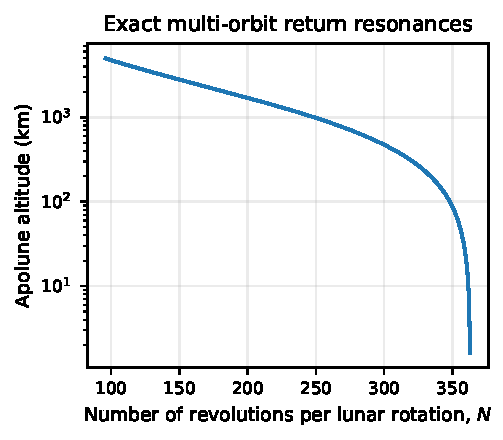
\includegraphics[width=0.47\textwidth]{fig08_rotation_resonances.pdf}
\caption{Ideal one-lunar-rotation resonances. The highest-order resonances are extremely low and terrain-sensitive; low-order resonances extend beyond the regime where a Moon-only model is credible.}
\label{fig:resonance}
\end{figure}

\subsection{Non-spherical lunar gravity}

Lunar gravity is not well approximated by a zonal $J_2$ alone. Mass concentrations and tesseral terms strongly affect low lunar orbits, motivating GRAIL models with hundreds to more than one thousand spherical-harmonic degrees \cite{Lemoine2014,Goossens2020}. Our packaged intermediate model retains the lowest non-spherical structure in a principal-axis frame:
\begin{align}
 U=\frac{\mu}{r}\bigg[1
 &-J_2\left(\frac{R}{r}\right)^2P_2(\sin\phi)\notag\\
 &+3C_{22}\left(\frac{R}{r}\right)^2\cos^2\phi\cos2\lambda\bigg].
\label{eq:degree2potential}
\end{align}
with representative unnormalised coefficients $J_2=2.033\times10^{-4}$ and $C_{22}=2.24\times10^{-5}$ consistent with lunar gravity solutions \cite{Williams2014}. Because the coefficients rotate with the Moon, the acceleration is evaluated in the body frame and transformed back to the inertial frame at every integration step.

For a representative equatorial eastward launch from \SI{20}{km} altitude, the inertial speed is $1.03$ times the local circular speed. Its central-gravity osculating period is \SI{7264.34}{s}, with an ideal apoapsis altitude of \SI{247.9}{km}. Table~\ref{tab:perturb} compares four models after that same reference period.

\begin{table*}[hbt]
\caption{One-reference-period propagation for the \SI{20}{km}-altitude test case. Position error is measured from the initial inertial position; site distance is measured from the rotated launch site. The degree-2 result is a controlled intermediate model, not a replacement for a high-degree GRAIL propagation.}
\label{tab:perturb}
\small
\resizebox{\textwidth}{!}{%
\begin{ruledtabular}
\begin{tabular}{lrrrr}
Model & Min. altitude (km) & Max. altitude (km) & Inertial error (km) & Site miss (km) \\
\hline
Central gravity & 20.000 & 247.932 & $1.0\times10^{-10}$ & 33.980 \\
Degree-2 Moon & 20.000 & 246.359 & 9.519 & 24.461 \\
Degree-2 + Earth & 20.000 & 246.298 & 9.560 & 24.420 \\
Degree-2 + Earth + Sun & 20.000 & 246.299 & 9.558 & 24.422
\end{tabular}
\end{ruledtabular}%
}
\end{table*}

The degree-2 correction at launch is about $4.95\times10^{-4}$ of central lunar gravity, while the Earth and solar differential tides are approximately $1.56\times10^{-5}$ and $4.39\times10^{-8}$ of central gravity. Yet the degree-2 term accumulates into a \SI{9.5}{km} mismatch after one ideal period. The Earth changes that particular short-arc result by tens of metres; the Sun is smaller still. These numbers are geometry-dependent, but they establish a defensible ordering of effects.

\begin{figure*}[hbt]
\centering
\subfigure[Altitude histories.]{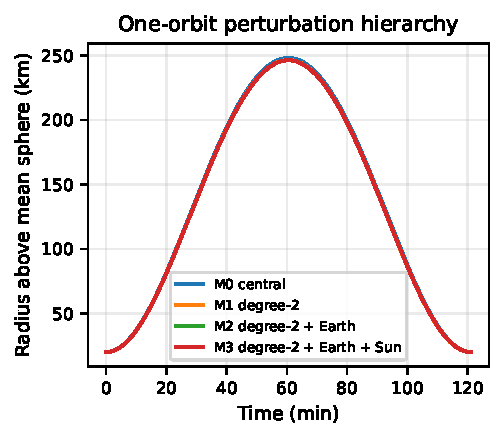
\includegraphics[width=0.47\textwidth]{fig09_perturbation_altitude.pdf}}
\hfill
\subfigure[Separation from the central model.]{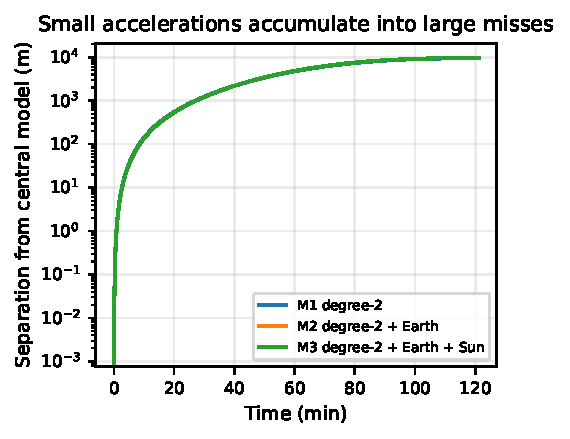
\includegraphics[width=0.47\textwidth]{fig10_perturbation_separation.pdf}}
\caption{Perturbation hierarchy for the representative \SI{20}{km} case. The Moon's own non-spherical gravity dominates the one-orbit correction; Earth tides are secondary over this short arc, and solar tides are smaller.}
\label{fig:perturb}
\end{figure*}

The existence of quasi-frozen low lunar orbits in spacecraft mission design does not rescue a literal one-swing home run automatically. Frozen orbits are selected orbital families whose averaged element variations are controlled, often with carefully chosen inclination, eccentricity, and argument of periapsis; they do not imply return to a particular rotating surface point without targeting and stationkeeping \cite{Folta2007,Ely2005}. The relevant conclusion is that a realistic lunar orbital home run is a precision trajectory-design problem, not a consequence of reaching one scalar speed.

\subsection{Third-body validity limits}

The differential acceleration from a third body at Moon-centred position $\vect R_j$ is
\begin{equation}
 \vect a_j=\mu_j\left[
 \frac{\vect R_j-\vect r}{|\vect R_j-\vect r|^3}
 -\frac{\vect R_j}{R_j^3}\right].
\label{eq:thirdbody}
\end{equation}
The indirect term is essential because the reference frame accelerates with the Moon. In low orbit and over one period, Earth tides are smaller than the degree-2 lunar correction. Near the escape boundary, however, the semimajor axis and period diverge, the trajectory approaches the scale of the Moon's gravitational sphere of influence, and Eq.~\eqref{eq:twobody} ceases to be a uniformly valid model. Consequently, ideal solutions with very long periods are mathematical continuations rather than physically credible lunar satellites.

\section{Analysis of the realistic solution}

\subsection{What is actually feasible?}

The word ``feasible'' has three different answers.

\emph{Human feasibility.} No. The speed deficit alone is a factor of 30.6, and no sensitivity refinement can bridge it.

\emph{Ideal launcher feasibility.} Yes. A tangential launch with $v_c\leq v<v_{\rm esc}$ produces a bound ideal orbit, and finite height gives a calculable angular tolerance. In the nonrotating model it returns exactly after one period.

\emph{Real lunar self-hit feasibility.} Only after trajectory targeting. A polar site removes the first-order rotation miss, while a nonpolar site requires a multi-orbit resonance or an intentionally non-Keplerian perturbed return. In either case, terrain and high-degree lunar gravity must be included. The launch state would have to be solved as a boundary-value problem,
\begin{equation}
 \vect F(\vect x_0,t_f)
 =\vect r(t_f;\vect x_0)-\vect r_{\rm site}(t_f)=\vect 0,
\label{eq:shooting}
\end{equation}
with collision constraints $C(t)>0$. A differential corrector or multiple-shooting method is appropriate; simply setting $v=v_c$ is not.

\subsection{Error budget and structural sensitivity}

Table~\ref{tab:error_budget} summarizes the roles of the main effects. The hierarchy depends on the chosen orbit, but several conclusions are robust: human speed is the dominant feasibility barrier; terrain and angular clearance dominate extremely low trajectories; lunar rotation dominates the difference between inertial and field return; and non-spherical lunar gravity dominates short-arc dynamical closure corrections over Earth and solar tides.

\begin{table*}[hbt]
\caption{Representative scale and consequence of each effect.}
\label{tab:error_budget}
\begin{ruledtabular}
\begin{tabular}{llll}
Effect & Representative scale & Primary consequence & Can it be ignored? \\
\hline
Human speed limit & $v_{\rm MLB}/v_c=0.0327$ & prevents orbital launch & no, for feasibility \\
Surface angle error & zero tolerance at $h=0$ & early impact & no, for ideal theorem \\
Finite \SI{1}{m} height & $|\gamma|_{\max}=0.034^\circ$ at $u=1.2$ & opens narrow safe set & no, for realism \\
Global terrain & $H_{\max}/R\simeq6.2\times10^{-3}$ & collision along ground track & no, in low orbit \\
Lunar rotation & \SI{30.05}{km} equatorial shift per $T_c$ & misses moving field & no, except at pole \\
Degree-2 gravity & $|a_2|/g\sim5\times10^{-4}$ & kilometre-scale closure error & no, for targeted return \\
Earth tide & $|a_E|/g\sim1.6\times10^{-5}$ & secondary short-arc correction & sometimes \\
Solar tide & $|a_S|/g\sim4.4\times10^{-8}$ & small over one low orbit & yes at first pass
\end{tabular}
\end{ruledtabular}
\end{table*}

The phrase ``measure-zero home run'' refers specifically to the $h=0$ M0 parameter space. It is not a claim that every realistic feasible set is mathematically measure zero. Finite launch height opens a small region, while targeting in a perturbed model can produce isolated solutions or narrow manifolds depending on which variables and terminal constraints are free. Maintaining that distinction avoids turning a useful theorem into an overstatement.

\subsection{Numerical validation}

The numerical trajectories are propagated with SciPy's DOP853 adaptive Runge--Kutta method \cite{Virtanen2020}. Before adding perturbations, the code integrates the analytic $u=1.2$ central orbit for exactly one closed-form period. Across maximum steps from \SI{2}{s} to \SI{60}{s}, the closure error remains below \SI{0.5}{\micro m}; relative energy and angular-momentum variations remain below $5\times10^{-14}$. The small non-monotonic variation in Fig.~\ref{fig:validation} is caused by adaptive tolerance and floating-point limits, not physical error. This test guards against attributing integrator drift to lunar perturbations.

\begin{figure}[hbt]
\centering
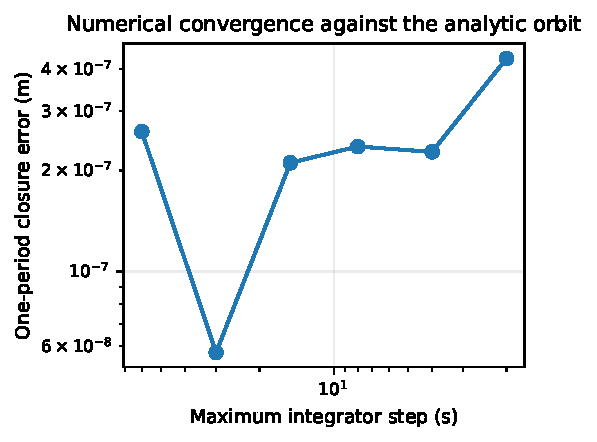
\includegraphics[width=0.47\textwidth]{fig12_numerical_convergence.pdf}
\caption{Central-orbit closure remains sub-micrometre across the tested maximum step sizes. The perturbation differences in Fig.~\ref{fig:perturb} are therefore many orders of magnitude larger than numerical closure error.}
\label{fig:validation}
\end{figure}

\subsection{Strengths and limitations}

The main strength of the approach is its separation of logically different questions. Existence is proven analytically; sensitivity is described by exact and asymptotic formulae; rotation is treated as a reference-frame problem; and realistic forces are added only after the numerical solver reproduces the analytic orbit. Every plotted quantity is regenerated from packaged scripts and saved as CSV.

Several limitations remain. First, the default non-spherical field is only degree 2. Real low lunar trajectories require a convergence study with GRGM900C or a later high-degree solution. Second, the optional terrain analysis uses a global grid and does not model rocks, crater rims below grid resolution, or uncertainty in the local vertical. Third, the fixed Earth/Sun directions are appropriate only for a short-arc scale comparison. Fourth, lunar libration and epoch-dependent attitude are omitted. Fifth, the collision is represented only through an initial velocity; bat deformation, launch spin, and launcher engineering are outside the orbital model. Finally, no stochastic high-degree gravity covariance is propagated, so the reported trajectory differences are model differences rather than formal confidence intervals.

These limitations suggest a clear next stage: use SPICE ephemerides and lunar orientation, propagate a filtered high-degree GRAIL field, query LOLA elevation along the body-fixed ground track, and solve Eq.~\eqref{eq:shooting} with a constrained differential corrector. The package is structured so that this extension can replace M3--M4 without changing the analytic M0--M1 foundation.

\section{Open problem: rules of baseball on the Moon}

Earth baseball rules assume a local field bounded by foul lines and an outfield fence; they do not define a ball that leaves the local neighbourhood, travels behind the field, and returns from another direction \cite{MLBRules2026}. A lunar rule set should separate competitive scoring from orbital safety.

\subsection{A three-dimensional fair region}

Two painted lines on a curved surface are insufficient once the ball can travel globally. We propose extending the foul rays from home plate into two half-planes containing the lunar centre. Their intersection defines a three-dimensional \emph{fair wedge}. A trajectory is fair at departure if its initial direction lies inside the wedge. After it crosses a certified stadium boundary, subsequent global longitude should not toggle the fair/foul decision repeatedly.

\subsection{An operational orbital-home-run criterion}

Waiting several hours or days for physical return would make play impossible. Instead, tracking radar or optical stations should estimate the osculating state immediately after the hit. An \emph{orbital home run} is declared if all of the following hold:
\begin{enumerate}
    \item the ball is fair at departure;
    \item its estimated trajectory is bound over the certified prediction horizon;
    \item the minimum predicted terrain clearance exceeds a safety margin;
    \item it crosses the stadium's three-dimensional outfield boundary without interception.
\end{enumerate}
Once declared, the ball becomes dead and all runners score. A returning ball cannot be caught for an out because the scoring decision has already been made. It must be collected by an autonomous capture system or deliberately deorbited into an unoccupied recovery zone.

\subsection{Three candidate ballparks}

\emph{Enclosed dome.} This is the safest and most Earth-like design. A roof prevents orbital debris, enables a breathable atmosphere, and restores familiar aerodynamic baseball. It also removes the orbital-home-run phenomenon.

\emph{Open field with an active capture shell.} A net or electromagnetic capture system above the field permits long lunar ballistic arcs but intercepts any ball whose speed exceeds a safety threshold. This design preserves distinctive lunar play without allowing uncontrolled satellites.

\emph{Polar research stadium.} A field near a rotation pole exploits the vanishing translational rotation miss and is the most scientifically interesting location for intentional orbital baseball. It requires terrain certification, high-degree gravity targeting, continuous tracking, and a protected return corridor. Competitive fairness would also require both teams to use the same launcher settings and field orientation, because azimuth relative to gravity anomalies matters.

A ball that genuinely circles the Moon should therefore count as a home run at the moment its safe orbital status is confirmed, not when it reappears. The rule makes scoring timely and prevents the returning ball from becoming a delayed weapon.

\section{Conclusion}

A lunar orbital home run is not characterized by one magic speed. In a smooth, nonrotating central field, the complete solution set for launch exactly from the surface is
\begin{equation*}
 \gamma=0,\qquad
 \SI{1.680}{km.s^{-1}}\leq v<\SI{2.376}{km.s^{-1}}.
\end{equation*}
This proves mathematical existence but also exposes structural fragility: the admissible speed--angle set has zero area. Finite ball-centre height changes the topology of the feasible set and gives an explicit angular tolerance; at \SI{1}{m} and $u=1.2$, the limit is \SI{0.0340}{deg}. A human hit nevertheless fails before precision becomes the main concern, because the best measured baseball exit speed is smaller than lunar circular speed by a factor of 30.6.

The phrase ``comes back'' must be defined in the correct frame. A near-surface ideal orbit closes in \SI{108.31}{min}, but an equatorial ballpark moves approximately \SI{30.05}{km} during that time. A polar field removes this first-order translational miss, and exact multi-orbit resonances exist in the ideal model, although their lowest-altitude members are threatened by real terrain. Mountains provide clearance but barely reduce the required speed.

Real lunar gravity qualitatively strengthens the caution. In the representative \SI{20}{km} case, a degree-2 field creates a \SI{9.5}{km} difference from one-period Kepler closure; Earth and solar tides are smaller over the same short arc. A credible self-hit must therefore be solved as a constrained, terrain-aware boundary-value problem using high-degree GRAIL gravity and LOLA topography. The final verdict is precise: an unaided batter cannot achieve an orbital home run; an engineered launcher can create ideal orbits; and a real return to the batter is possible only as an actively targeted astrodynamics experiment, preferably at a polar, instrumented, safety-controlled ballpark.

\appendix

\section{Derivation of the arbitrary-height boundary}

At launch,
\begin{equation}
 \mathcal E=\frac{v^2}{2}-\frac{\mu}{r_0},\qquad
 H=r_0v\cos\gamma.
\end{equation}
At the limiting periapsis $R_t$, radial speed vanishes and tangential speed is $H/R_t$, giving
\begin{equation}
 \mathcal E=\frac{H^2}{2R_t^2}-\frac{\mu}{R_t}.
\end{equation}
Equating the two expressions and inserting $H$ yields Eq.~\eqref{eq:height_boundary}. The denominator in Eq.~\eqref{eq:vmin} requires $r_0|\cos\gamma|>R_t$; geometrically, the initial angular momentum must be large enough that a tangent from the launch point can clear the obstacle sphere.

\section{Coordinate construction}

At body-fixed latitude $\phi$ and longitude $\lambda$, the local unit vectors are
\begin{align}
 \hat{\vect e}_r&=(\cos\phi\cos\lambda,\cos\phi\sin\lambda,\sin\phi),\\
 \hat{\vect e}_E&=(-\sin\lambda,\cos\lambda,0),\\
 \hat{\vect e}_N&=(-\sin\phi\cos\lambda,-\sin\phi\sin\lambda,\cos\phi).
\end{align}
For azimuth $A$ clockwise from north,
\begin{equation}
 \vect v_s=v_s\left[\cos\gamma(\cos A\,\hat{\vect e}_N+\sin A\,\hat{\vect e}_E)+\sin\gamma\,\hat{\vect e}_r\right].
\end{equation}
Equation~\eqref{eq:rotation_velocity} then produces the Moon-centred inertial initial condition.

\section{Reproducibility}

The accompanying project archive contains the full \LaTeX{} source, compiled PDF, Python scripts, generated figures, input constants, optional-data manifest, and all tabulated outputs. Running
\begin{verbatim}
python scripts/generate_all.py
cd docs && latexmk -pdf main.tex
\end{verbatim}
regenerates the default results. Large LOLA and GRAIL products are intentionally not duplicated; their official NASA PDS URLs and a download script are provided under \texttt{data/input} and \texttt{scripts}. The default paper therefore remains reproducible offline after installation of the listed Python packages, while the high-fidelity extension remains traceable to authoritative data.

\bibliography{references}

\end{document}
